\documentclass[tikz, border=6pt]{standalone}
\usepackage[T1]{fontenc}
\usepackage{lmodern}
\usepackage{amsmath,amssymb,bm}
\usepackage[scaled=0.95]{helvet}
\usetikzlibrary{arrows.meta}
\definecolor{Blue}{HTML}{3A76D8}
\definecolor{Green}{HTML}{3BA55C}
\definecolor{Orange}{HTML}{EE8133}
\definecolor{Red}{HTML}{DF4B4B}
\definecolor{Ink}{HTML}{1F2937}
\colorlet{softmax}{Green}
\tikzset{
  neuron/.style={/utils/exec={\colorlet{pytikzarg}{#1}}, circle, draw=pytikzarg!78!black, fill=pytikzarg!22, minimum size=7.2mm, inner sep=0pt, line width=0.7pt, font=\small},
  neuron/.default=Blue,
  connection/.style={Ink!38, line width=0.45pt, -{Stealth[length=3.2pt, width=2.6pt]}, shorten >=1pt},
  layer title/.style={font=\small\bfseries, align=center},
}
\begin{document}
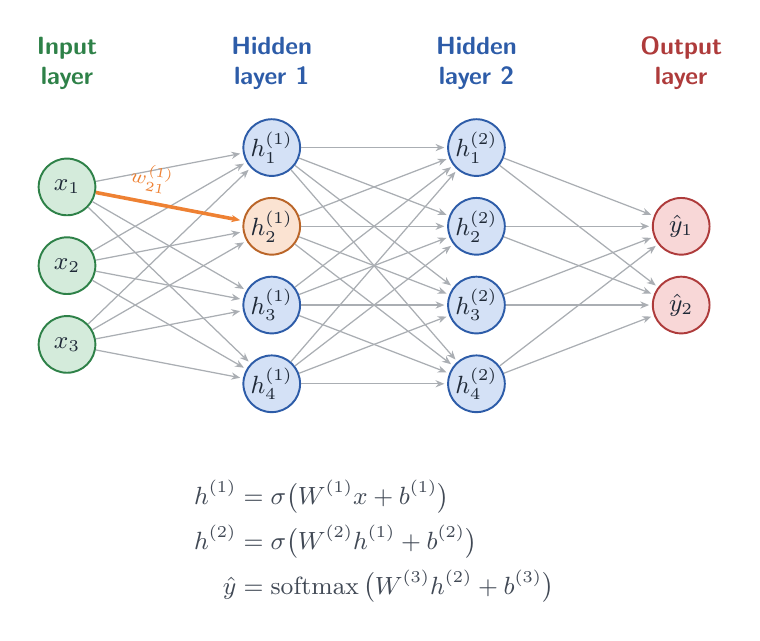
\begin{tikzpicture}[color=Ink, execute at begin picture={\sffamily}, line width=0.6pt, >={Stealth[length=5.5pt, width=4pt, inset=1.2pt]}, line join=round]
  % neural network nn: 3-4-4-2
  \node[neuron=Green] (nn-0-0) at (0,1) {$x_{1}$};
  \node[neuron=Green] (nn-0-1) at (0,0) {$x_{2}$};
  \node[neuron=Green] (nn-0-2) at (0,-1) {$x_{3}$};
  \node[neuron=Blue] (nn-1-0) at (2.6,1.5) {$h^{(1)}_{1}$};
  \node[neuron=Orange] (nn-1-1) at (2.6,0.5) {$h^{(1)}_{2}$};
  \node[neuron=Blue] (nn-1-2) at (2.6,-0.5) {$h^{(1)}_{3}$};
  \node[neuron=Blue] (nn-1-3) at (2.6,-1.5) {$h^{(1)}_{4}$};
  \node[neuron=Blue] (nn-2-0) at (5.2,1.5) {$h^{(2)}_{1}$};
  \node[neuron=Blue] (nn-2-1) at (5.2,0.5) {$h^{(2)}_{2}$};
  \node[neuron=Blue] (nn-2-2) at (5.2,-0.5) {$h^{(2)}_{3}$};
  \node[neuron=Blue] (nn-2-3) at (5.2,-1.5) {$h^{(2)}_{4}$};
  \node[neuron=Red] (nn-3-0) at (7.8,0.5) {$\hat y_{1}$};
  \node[neuron=Red] (nn-3-1) at (7.8,-0.5) {$\hat y_{2}$};
  \draw[connection] (nn-0-0) -- (nn-1-0);
  \draw[connection] (nn-0-0) -- (nn-1-2);
  \draw[connection] (nn-0-0) -- (nn-1-3);
  \draw[connection] (nn-0-1) -- (nn-1-0);
  \draw[connection] (nn-0-1) -- (nn-1-1);
  \draw[connection] (nn-0-1) -- (nn-1-2);
  \draw[connection] (nn-0-1) -- (nn-1-3);
  \draw[connection] (nn-0-2) -- (nn-1-0);
  \draw[connection] (nn-0-2) -- (nn-1-1);
  \draw[connection] (nn-0-2) -- (nn-1-2);
  \draw[connection] (nn-0-2) -- (nn-1-3);
  \draw[connection] (nn-1-0) -- (nn-2-0);
  \draw[connection] (nn-1-0) -- (nn-2-1);
  \draw[connection] (nn-1-0) -- (nn-2-2);
  \draw[connection] (nn-1-0) -- (nn-2-3);
  \draw[connection] (nn-1-1) -- (nn-2-0);
  \draw[connection] (nn-1-1) -- (nn-2-1);
  \draw[connection] (nn-1-1) -- (nn-2-2);
  \draw[connection] (nn-1-1) -- (nn-2-3);
  \draw[connection] (nn-1-2) -- (nn-2-0);
  \draw[connection] (nn-1-2) -- (nn-2-1);
  \draw[connection] (nn-1-2) -- (nn-2-2);
  \draw[connection] (nn-1-2) -- (nn-2-3);
  \draw[connection] (nn-1-3) -- (nn-2-0);
  \draw[connection] (nn-1-3) -- (nn-2-1);
  \draw[connection] (nn-1-3) -- (nn-2-2);
  \draw[connection] (nn-1-3) -- (nn-2-3);
  \draw[connection] (nn-2-0) -- (nn-3-0);
  \draw[connection] (nn-2-0) -- (nn-3-1);
  \draw[connection] (nn-2-1) -- (nn-3-0);
  \draw[connection] (nn-2-1) -- (nn-3-1);
  \draw[connection] (nn-2-2) -- (nn-3-0);
  \draw[connection] (nn-2-2) -- (nn-3-1);
  \draw[connection] (nn-2-3) -- (nn-3-0);
  \draw[connection] (nn-2-3) -- (nn-3-1);
  \draw[connection, Orange, line width=1.3pt] (nn-0-0) -- node[pos=0.35, sloped, above, font=\scriptsize, text=Orange] {$w^{(1)}_{21}$} (nn-1-1);
  \node[layer title, anchor=south, text=Green!78!black] (nn-title-0) at (0,2.11) {Input\\layer};
  \node[layer title, anchor=south, text=Blue!78!black] (nn-title-1) at (2.6,2.11) {Hidden\\layer 1};
  \node[layer title, anchor=south, text=Blue!78!black] (nn-title-2) at (5.2,2.11) {Hidden\\layer 2};
  \node[layer title, anchor=south, text=Red!78!black] (nn-title-3) at (7.8,2.11) {Output\\layer};
  \node[anchor=north, font=\small, text=Ink!85] at (3.9,-2.6) {$\begin{aligned}
    h^{(1)} &= \sigma\big(W^{(1)}x + b^{(1)}\big)\\
    h^{(2)} &= \sigma\big(W^{(2)}h^{(1)} + b^{(2)}\big)\\
    \hat y  &= \operatorname{softmax}\big(W^{(3)}h^{(2)} + b^{(3)}\big)
  \end{aligned}$};
\end{tikzpicture}
\end{document}
